\documentclass{article}
% Bold vector notation was applied with AI assistance.
\usepackage[en]{homework}
\usepackage{tikz}
\usepackage{needspace}
\usetikzlibrary{arrows.meta}

\config{Physics-1}{2026 Fall}{5}

\begin{document}

\begin{problem}
From the definition of cross product and inner product, show that
\begin{enumerate}
  \item[(a)] $\bo{a}\times(\bo{b}\times\bo{c})=\bo{b}(\bo{c}\cdot\bo{a})-\bo{c}(\bo{a}\cdot\bo{b})$.
  \item[(b)] $\bo{a}\cdot(\bo{b}\times\bo{c})=\bo{b}\cdot(\bo{c}\times\bo{a})=-\bo{c}\cdot(\bo{b}\times\bo{a})$.
\end{enumerate}
\end{problem}

\begin{proof}
	\paragraph{(a)} Using the Einstein summation convention, the cross product can be expanded as
	\begin{align*}
		\bo{a} \times (\bo{b} \times \bo{c}) 
		&= \varepsilon_{ijk} \bo{e}_i a_j (\bo{b} \times \bo{c})_k
		= \varepsilon_{ijk}\varepsilon_{klm} \bo{e}_i a_j b_l c_m \\
		&= (\delta_{il} \delta_{jm} - \delta_{im} \delta_{jl}) \bo{e}_i a_j b_l c_m
		= \bo{e}_i b_i a_j c_j - \bo{e}_i c_i a_j b_j \\
		&= \bo{b}(\bo{c} \cdot \bo{a}) - \bo{c} (\bo{a} \cdot \bo{b}).
	\end{align*}

	\paragraph{(b)} Indeed, 
	\[ \bo{a} \cdot (\bo{b} \times \bo{c}) = a_i (\bo{b} \times \bo{c})_i = \varepsilon_{ijk} a_i b_j c_k. \]
	Similarly, $\bo{b} \cdot (\bo{c} \times \bo{a}) = \bo{c} \cdot (\bo{a} \times \bo{b}) = \varepsilon_{ijk} a_i b_j c_k$.
\end{proof}



\begin{problem}
A uniform solid cylinder lies on top of a board. There is sufficient static friction between the cylinder and the board to prevent slipping. The board is placed on a table. The cylinder and the board have the same mass $m$, and the coefficient of kinetic friction between the board and the table is $\mu_k$. Initially, both the cylinder and the board have velocity $v_0$.
\begin{enumerate}
  \item[(a)] What is the acceleration of the board?
  \item[(b)] What is the speed of the cylinder when the board comes to a stop?
\end{enumerate}
\begin{center}
  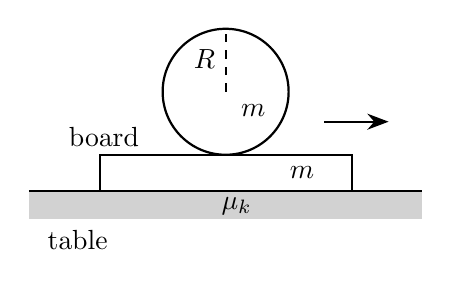
\begin{tikzpicture}[line width=.8pt, >=Stealth, font=\normalfont\normalsize]
  \fill[gray!35] (0,-.36) rectangle (5,0);
  \draw (0,0) -- (5,0);
  \draw (.9,0) rectangle (4.1,.46);
  \draw (2.5,1.26) circle[radius=.8];
  \draw[dashed] (2.5,1.26) -- (2.5,2.06);
  \node at (2.23,1.68) {$R$};
  \node at (2.85,1.02) {$m$};
  \node at (3.47,.23) {$m$};
  \node[anchor=east] at (1.53,.69) {board};
  \node at (.62,-.62) {table};
  \node at (2.64,-.19) {$\mu_k$};
  \draw[-{Stealth[length=2.7mm]}] (3.75,.88) -- (4.57,.88);
\end{tikzpicture}

\end{center}
\end{problem}

\begin{solution}
	\paragraph{(a)} The kinetic friction between the table and borad is
	\[ f_1 = \mu_k (m + m)g = 2\mu_k mg. \]
	Denote the clockwise angular acceleration of the cylinder by $\alpha$, and the decelerations of the board and the cylinder by $a_{\mathrm{b}}$ and $a_{\mathrm{c}}$. The no-slip condition gives
	\[ a_{\mathrm{c}} = a_{\mathrm{b}} - R\alpha. \]
	Suppose that the friction between the board and the cylinder is $f_2$. By Newton's law, 
	\[ \begin{cases}
		f_1 - f_2 = m a_{\mathrm{b}}, \\
		f_2 = m a_{\mathrm{c}}, \\
		Rf_2 = I \alpha,
	\end{cases} \]
	where $I = mR^2/2$ is the inertia of rotation of the cylinder. By solving this equation, we got
	\[ a_{\mathrm{b}} = \frac{3}{2}\mu_k g, \qquad a_{\mathrm{c}} = \frac{1}{2}\mu_k g, \qquad \alpha = \frac{\mu_k g}{R}, \qquad f_2 = \frac{1}{2}\mu_k mg. \]
	
	Therefore, the acceleration of the board is $a_{\mathrm{b}} = 3 \mu_k g/2$.

	\paragraph{(b)} Suppose that it takes time $t$ for the board to come to a stop. The final velocity of the cylinder is $v := v_0 - a_{\mathrm{c}}t$. Combining with $v_0 - a_{\mathrm{b}} t = 0$ and the previous results, we got 
	\[ v = v_0 - a_{\mathrm{c}}\frac{v_0}{a_{\mathrm{b}}} = \left(1 - \frac{1}{3}\right)v_0 = \frac{2}{3}v_0. \]
\end{solution}



\begin{problem}
A uniform thin rod of mass $M$ and length $L$ is initially held at rest, leaning against a vertical wall at an angle $\theta_0$ with the horizontal floor, where $0<\theta_0<\pi/2$. Both the wall and the floor are frictionless. The rod is then released.
\begin{enumerate}
  \item[(a)] While both ends remain in contact with the wall and floor, find the angular speed of the rod as a function of the angle $\theta$ it makes with the horizontal.
  \item[(b)] Find the normal force exerted by the wall on the rod as a function of $\theta$.
  \item[(c)] Show that the upper end of the rod loses contact with the wall before reaching the floor. Find the angle at which this happens.
\end{enumerate}
\end{problem}

\begin{solution}
	\paragraph{(a)} From the geometry relation, we know that while the rod is at angle $\theta$ and angular speed $\omega$, the height of the center of mass is $(L/2) \sin \theta$, and the velocity of the center of mass is $(L/2) \omega$. The kinetic energy can be written as
	\[ E_k = E_{\mathrm{rotation}} + E_{\mathrm{translation}} = \frac{ML^2}{24} \omega^2 + \frac{ML^2}{8} \omega^2 = \frac{ML^2}{6} \omega^2. \]

	Accroding to the conservation of energy, the kinetic energy comes from the loss of potential energy of gravity, which is
	\[ E_k = \frac{MgL}{2}(\sin \theta_0 - \sin \theta). \]

	Therefore, 
	\[ \omega = \sqrt{\frac{3g}{L}(\sin \theta_0 - \sin \theta)}. \]

	\paragraph{(b)} Since $\theta$ decreases during the motion, $\dot\theta = -\omega$. Differentiating the relation in (a), we have
	\[ 2\dot\theta\ddot\theta = -\frac{3g}{L}\cos\theta\dot\theta \implies \ddot\theta = -\frac{3g}{2L}\cos\theta. \]
	Take the direction away from the wall as the positive horizontal direction. The horizontal position of the center of mass is $x_{\mathrm{CM}} = (L/2)\cos\theta$. Therefore,
	\begin{align*}
		a_x = \ddot x_{\mathrm{CM}}
		&= -\frac{L}{2}\left(\cos\theta\dot\theta^2 + \sin\theta\ddot\theta\right) \\
		&= \frac{3g}{4}\cos\theta(3\sin\theta - 2\sin\theta_0).
	\end{align*}
	The normal force from the wall is the only horizontal external force, so
	\[ N = Ma_x = \frac{3Mg}{4}\cos\theta(3\sin\theta - 2\sin\theta_0). \]

	\paragraph{(c)} The wall can only push the rod, so $N \ge 0$. The upper end loses contact with the wall when $N = 0$. Since $\cos\theta > 0$, we get
	\[ 3\sin\theta - 2\sin\theta_0 = 0 \implies \theta = \arcsin\left(\frac{2}{3}\sin\theta_0\right). \]
	This angle satisfies $0 < \theta < \theta_0$, so the upper end loses contact with the wall before reaching the floor.
\end{solution}



\begin{problem}
Two identical uniform disks are rotating with the same angular velocity $\omega$. Glue was applied to the side of the disks. Initially the two disks are slightly separated, but you give a gentle push to the disks so that they come into contact and stick together.
\begin{enumerate}
  \item[(a)] What is the angular velocity of the resulting system?
  \item[(b)] How much kinetic energy is lost?
\end{enumerate}
\begin{center}
  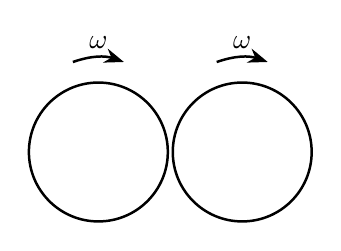
\begin{tikzpicture}[scale=.9, line width=.9pt, >=Stealth, font=\normalfont\normalsize]
  \foreach \x in {0,2.03} {
    \draw (\x,0) circle[radius=.98];
    \draw[->] (\x-.36,1.27) to[bend left=19] (\x+.36,1.27);
    \node at (\x,1.54) {$\omega$};
  }
\end{tikzpicture}

\end{center}
\end{problem}

\begin{solution}
	\paragraph{(a)} Denote the mass and the radius of each disk by $m$ and $R$, respectively. The initial angular momentum is
	\[ L = 2I\omega = 2 \cdot \frac{1}{2}mR^2\omega = mR^2\omega. \]
	By the parallel axis theorem, the moment of inertia of the resulting system is
	\[ I_{\mathrm{total}} = 2(I + mR^2) = 3mR^2. \]
	From angular momentum conservation, we have
	\[ 2I\omega = I_{\mathrm{total}}\omega' \implies \omega' = \frac{1}{3}\omega. \]

	\paragraph{(b)} The kinetic energies before and after the disks stick together are
	\begin{gather*}
		E_k = 2 \cdot \frac{1}{2}I\omega^2 = \frac{1}{2}mR^2\omega^2, \\
		E_k' = \frac{1}{2}I_{\mathrm{total}}(\omega')^2
		= \frac{3}{2}mR^2 \cdot \frac{\omega^2}{9}
		= \frac{1}{6}mR^2\omega^2.
	\end{gather*}
	Therefore, the loss of kinetic energy is
	\[ \Delta E_k = \frac{1}{3}mR^2\omega^2. \]
\end{solution}



\Needspace{8cm}
\begin{problem}
A ball initially slides without rotating on a horizontal surface with friction. The initial speed of the ball is $V_0$, and the moment of inertia about its center is $I=\eta mR^2$.
\begin{enumerate}
  \item[(a)] Without knowing anything about the nature of the friction force, find the speed of the ball when it begins to roll without slipping. Also, find the kinetic energy lost while sliding.
  \item[(b)] Now consider the special case where the coefficient of kinetic friction is $\mu$, independent of position. At what time, and at what distance, does the ball begin to roll without slipping? Verify that the work done by friction equals the energy loss calculated in part (a). (Be careful on this.)
\end{enumerate}
\begin{center}
  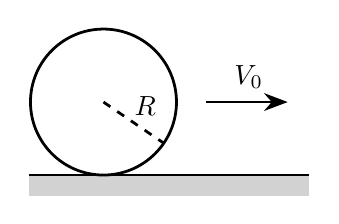
\begin{tikzpicture}[scale=.9, line width=1pt, >=Stealth, font=\normalfont\normalsize]
  \fill[gray!35] (.35,-.3) rectangle (4.3,0);
  \draw (.35,0) -- (4.3,0);
  \draw (1.4,1.03) circle[radius=1.03];
  \draw[dashed] (1.4,1.03) -- (2.25,.45);
  \node at (1.99,.98) {$R$};
  \draw[-{Stealth[length=3mm]}] (2.85,1.03) -- (4.0,1.03);
  \node at (3.45,1.38) {$V_0$};
\end{tikzpicture}

\end{center}
\end{problem}

\begin{solution}
	Denote $\omega_0 = V_0/R$. Initially, $L_0 = 0$. When the ball begins to roll without slipping, we have $\omega = V/R$ and $L = I\omega$.

	\paragraph{(a)} Let $f$ denote the friction. From the changes in momentum and angular momentum, we have
	\[ m(V_0 - V) = \int f \d t, \qquad I\omega = R\int f \d t. \]
	Using $I = \eta mR^2$ and $\omega = V/R$, we get
	\[ V = \frac{V_0}{1 + \eta}. \]
	The initial and final kinetic energies are
	\[ E_{k0} = \frac{1}{2}mV_0^2, \qquad E_k = \frac{1}{2}mV^2 + \frac{1}{2}I\omega^2. \]
	Therefore, the loss of kinetic energy is
	\[ \Delta E_k = \frac{\eta}{1 + \eta} \cdot \frac{1}{2}mV_0^2. \]

	\paragraph{(b)} In this case, $f = \mu mg$, so
	\[ I\omega = Rtf \implies t = \frac{I\omega}{Rf} = \frac{\eta V_0}{(1 + \eta)\mu g}. \]
	The distance is
	\[ x = \frac{V_0^2 - V^2}{2\mu g} = \frac{V_0^2\eta(\eta + 2)}{2\mu g(1 + \eta)^2}. \]
	The relative displacement between the ball and the surface is
	\[ \Delta x = x - \int_0^t R\omega(t)\d t = \frac{V_0^2\eta}{2\mu g(\eta + 1)}. \]
	Then the magnitude of the work done by the friction is
	\[ W_f = \frac{\eta}{1 + \eta} \cdot \frac{1}{2}mV_0^2 = \Delta E_k. \]
\end{solution}



\Needspace{8cm}
\begin{problem}
A disk of mass $M$ and radius $R$ unwinds from a tape wrapped around it. The tape passes over a frictionless pulley, and a mass $m$ is suspended from the other end. Assume that the disk drops vertically.
\begin{enumerate}
  \item[(a)] Relate the accelerations of $m$ and the disk, $a$ and $A$, respectively, to the angular acceleration $\alpha$ of the disk.
  \item[(b)] Find $a$, $A$, and $\alpha$.
\end{enumerate}
\begin{center}
  \resizebox{!}{4.1cm}{\begin{tikzpicture}[line width=.65pt, >=Stealth, font=\normalfont\normalsize]
  % The tape and the two circular bodies share the source's oblique view.
  % Background-coloured fills hide only the lines behind solid objects.
  \draw[fill=shadecolor] (-1.25,.95) -- (-.63,1.3) -- (-.23,1.08)
    -- (-.23,.36) -- (-.85,0) -- (-1.25,.22) -- cycle;
  \draw (-1.25,.95) -- (-.85,.72) -- (-.23,1.08);
  \draw (-.85,.72) -- (-.85,0);
  \node at (-.52,.54) {$m$};

  \draw[fill=shadecolor] (-.98,3.3) -- (-.66,3.46)
    -- (-.66,1.3) -- (-.98,1.1) -- cycle;
  \draw[fill=shadecolor] (.98,3.3) -- (1.30,3.46)
    -- (1.30,.43) -- (.98,.25) -- cycle;

  % Rear part of the pulley axle.
  \draw[fill=shadecolor, rounded corners=.025cm]
    (.25,3.39) -- (1.56,4.15) -- (1.61,4.06) -- (.30,3.30) -- cycle;
  \draw[fill=shadecolor] (.32,3.46) ellipse[x radius=.98,y radius=1.05];
  \draw[fill=shadecolor] (0,3.3) ellipse[x radius=.98,y radius=1.05];
  % Front part of the axle, in front of the pulley face.
  \draw[fill=shadecolor, rounded corners=.035cm]
    (-1.43,2.43) -- (-.02,3.25) -- (.03,3.34)
    -- (-.02,3.4) -- (-1.48,2.55) -- cycle;

  \draw[fill=shadecolor] (2.62,.43) ellipse[x radius=1.28,y radius=1.35];
  \draw[fill=shadecolor] (2.25,.25) ellipse[x radius=1.28,y radius=1.35];
  \node at (1.57,.86) {$M$};
  \draw[-{Stealth[length=1.7mm,width=1.2mm]},line width=.45pt]
    (2.25,.25) -- (1.42,-.63);
  \node at (1.67,.10) {$R$};
  \draw[-{Stealth[length=2.4mm]},line width=1.5pt]
    (2.25,.25) -- (2.25,-.87);
  \node at (2.51,-.57) {$A$};
  \draw[->] (2.49,1.26) arc[start angle=75,end angle=0,x radius=.94,y radius=1.04];
  \node at (2.93,.11) {$\alpha$};

  \draw[-{Stealth[length=2.4mm]},line width=1.4pt]
    (-.82,-.10) -- (-.82,-.89);
  \node at (-.57,-.48) {$a$};
  \draw[-{Stealth[length=2.4mm]},line width=1.4pt]
    (2.62,3.68) -- (2.62,2.88);
  \node at (2.88,3.28) {$g$};
\end{tikzpicture}
}
\end{center}
\end{problem}

\begin{solution}
	\paragraph{(a)} Take the downward direction as positive for both $x_m$ and $x_{\mathrm{CM}}$, and take the clockwise direction as positive for $\theta$. Since the length of the tape is fixed, we have
	\[ x_m + x_{\mathrm{CM}} - R\theta = \mathrm{const} \implies a + A - R\alpha = 0. \]

	\paragraph{(b)} Let $T$ denote the tension in the tape. From Newton's laws, we have
	\[
		\begin{cases}
			mg - T = ma, \\
			Mg - T = MA, \\
			TR = \frac{1}{2}MR^2\alpha.
		\end{cases}
	\]
	Solving these equations together with the relation in (a), we get
	\[
		\begin{cases}
			a = \dfrac{3m - M}{3m + M}g, \\[7pt]
			A = \dfrac{m + M}{3m + M}g, \\[7pt]
			\alpha = \dfrac{4m}{3m + M}\dfrac{g}{R}.
		\end{cases}
	\]
\end{solution}

\end{document}
